\section{Empirical analysis of improvement}

In order to empirically assess the space efficiency of our improvement, we
measured the size of the interlink data structure in the case of interlink
\emph{lists}, the previously proposed format, and in the case of interlink
\emph{sets}, our newly proposed format. We performed our measurements on the
mainnet for both Bitcoin and Litecoin. Our results are illustrated in
Figure~\ref{fig.set-list-vector-comparison} and are similar for both of these
coins.

The new data structure format yields savings of approximately $83\%$ on average.
Based on the theoretical analysis of Section~\ref{sec.construction}, we expect
to see approximately an improvement of $50\%$ in this structure. The extra
$33\%$ is due to the explosion of difficulty in the mining power in both
cryptocurrencies. The increased difficulty causes a lower variable difficulty
target, meaning that the lowest portions of the superblock levels remain
unoccupied, but are still accounted for in the interlink vector list approach.

\begin{figure}
   \centering
   \subcaptionbox[]{%
      \centering
      Bitcoin
   }
   [
       0.80\textwidth
   ]
   {
       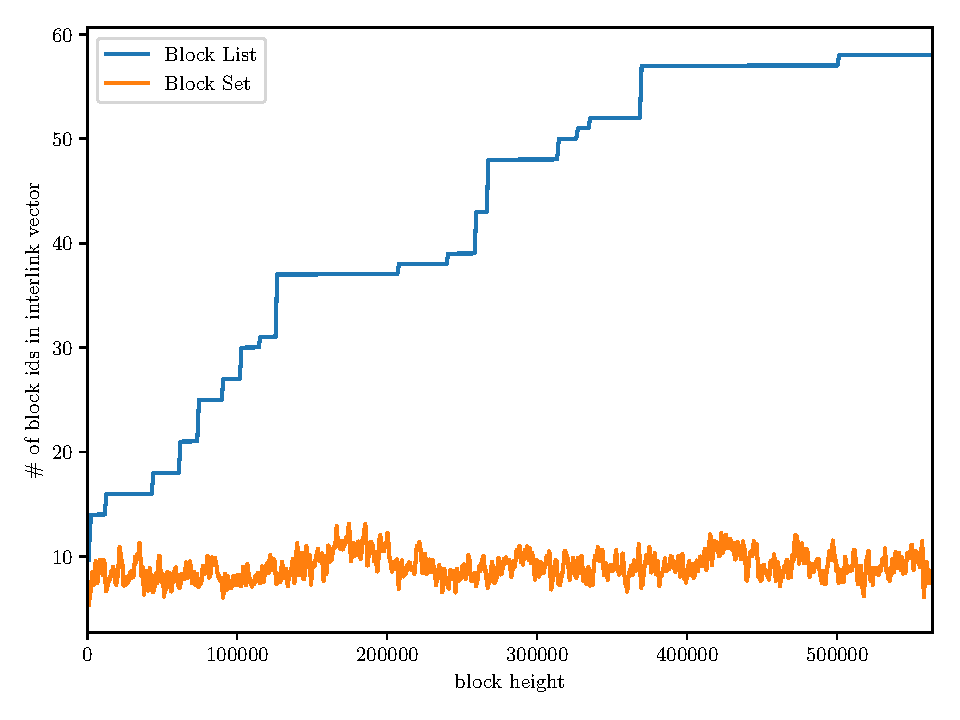
\includegraphics[width=0.85 \textwidth]
       {figures/interlink-vector-blocklist-vs-blockset.pdf}
   }
   \vskip 0pt
   \subcaptionbox[]{%
      \centering
      Litecoin
   }
   [
       0.80\textwidth
   ]
   {
       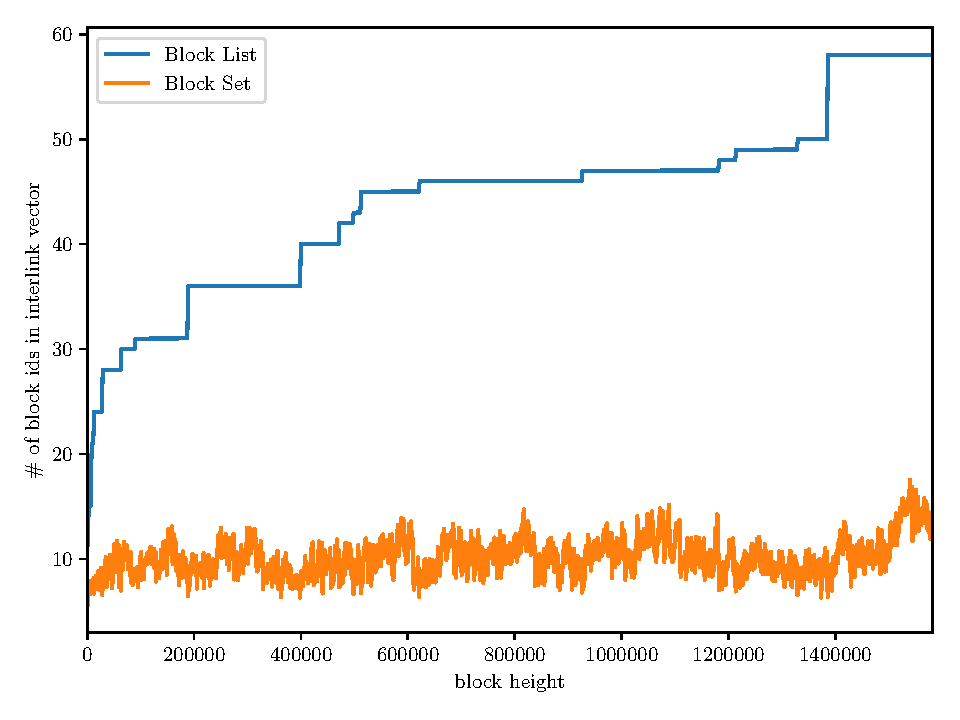
\includegraphics[width=0.85 \textwidth]
       {figures/interlink-vector-blocklist-vs-blockset-litecoin.pdf}
   }
   \caption{A comparison of interlink vector sizes for interlink block lists (previous work) and interlink block sets (this work) in two popular blockchains (lower is better)}
   \label{fig.set-list-vector-comparison}
\end{figure}

Based on the sizes attained in the interlink vector, we organized the interlink
vector into Merkle trees for both the list and the set structure and created
proofs-of-inclusion of which we measured the size. Our results are illustrated
in Figure~\ref{fig.set-list-proof-comparison}.

\begin{figure*}[h]
\begin{center}
  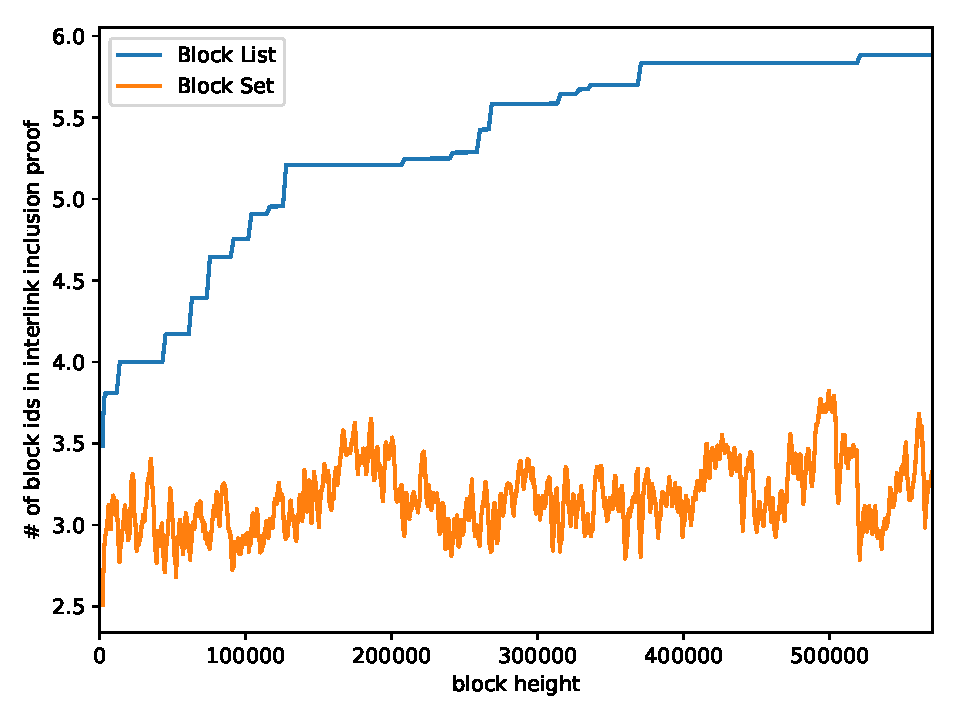
\includegraphics[width=0.95\textwidth]{figures/interlink-proof-list-vs-set.pdf}
  \caption{A comparison of a proof-of-inclusion size in the case of interlink block lists (previous work) and interlink block sets (this work) in Bitcoin (lower is better)}
  \label{fig.set-list-proof-comparison}
  \end{center}
\end{figure*}

\begin{figure*}[h]
\begin{center}
  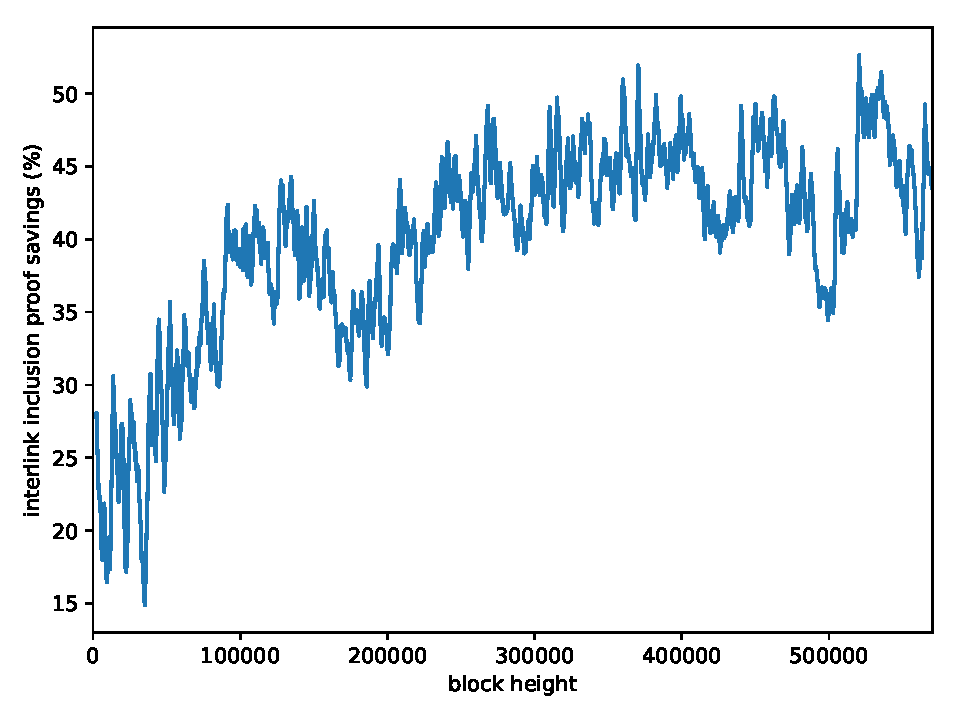
\includegraphics[width=0.95\textwidth]{figures/interlink-proof-savings-from-blockset.pdf}
  \caption{Percentile savings of our block set construction compared to the
           previously known block list construction.}
  \label{fig.set-list-proof-comparison}
  \end{center}
\end{figure*}

\TODO{TODO: Explain Figure~\ref{fig.set-list-proof-comparison}}

\begin{table}[h!]
  \begin{center}
    \begin{tabular}{|c|cc|cc|cc|}
      \hline
      & \multicolumn{2}{c|}{\bf Interlink size}
      & \multicolumn{2}{c|}{\bf Proof-of-inclusion size}
      & \multicolumn{2}{c|}{\bf NIPoPoW size}\\
      & blocks & bytes & blocks & bytes & blocks & bytes\\
      \hhline{-------}
      \textbf{Interlink lists}&
      5 & 7 & 35 & 25 & 0 & 1\\
      \hline
      \makecell{\bf Interlink sets\\(this work)}&
      5 & 7 & 35 & 25 & 0 & 1\\
      \hline
    \end{tabular}
    \vspace{10pt}
    \caption{A comparison of the two interlink constructions in terms of size.}
    \label{tab:overview}
  \end{center}
\end{table}

\TODO{TODO fill in exact numbers in above table}
\TODO{TODO explain above table results and methodology}
